\section{Models, Task Evaluation, and Prompts}\label{appendix:task-evaluation-prompts}
\subsection{Models}
We use DeepSeek \citep{guo2024deepseek}, CodeLlama \citep{roziere2023code}, and StarCoder \citep{li2023starcoder} models. The HuggingFace URLs are listed in Table \ref{tab:model-url-list}. Experiments were run on A100 (80 GB) and A6000 (40 GB) machines.
\begin{table}[h]
    \centering
    \small
    \caption{Model Links}
    \begin{tabular}{|ll|}
        \hline
        \textbf{Model Name} & \textbf{HuggingFace URL} \\
        \hline
        DeepSeek Instruct (6.7B) & \url{https://huggingface.co/deepseek-ai/deepseek-coder-6.7b-instruct} \\
        DeepSeek Instruct (33B) & \url{https://huggingface.co/deepseek-ai/deepseek-coder-33b-instruct} \\
        StarCoder (15.5B) & \url{https://huggingface.co/bigcode/starcoder} \\
        CodeLlama (7B) & \url{https://huggingface.co/codellama/CodeLlama-7b-hf} \\
        CodeLlama (13B) & \url{https://huggingface.co/codellama/CodeLlama-13b-hf} \\
        CodeLlama (34B) & \url{https://huggingface.co/codellama/CodeLlama-34b-hf} \\
        CodeLlama Instruct (34B) & \url{https://huggingface.co/codellama/CodeLlama-34b-Instruct-hf} \\
        \hline
    \end{tabular}
    \label{tab:model-url-list}
\end{table}


\subsection{Task Evaluation}
\label{sec:task-eval}
\textit{Correctness Checking}: For this task, we use an autoregressive-style CoT prompt from Listing \ref{lst:correctness-checking-prompt-cot}. We perform majority voting on the binary label (correct/incorrect) with $N=10$ samples and temperature $T=0.2$ and report accuracy on these labels. We do this because greedy decoding can be noisy for chain-of-thought prompting and majority voting has been shown to help \citep{wei2022chain, wang2022self}.

We also compared this with an autoregressive-style prompt without CoT, where the model is simply asked to predict Correct/Incorrect. In this case, we have the direct log-probabilities of each outcome $p_{\text{correct}}$ and $p_{\text{incorrect}} = 1 - p_{\text{correct}}$, so the predicted label is taken to be $p_{\text{correct}} \ge 0.5$. In Fig. \ref{fig:correctness-checking-cot-impact}, we observe that for a majority of settings and samples, CoT helps the accuracy of this task, motivating our use of CoT.

\begin{figure}[H]
    \centering
    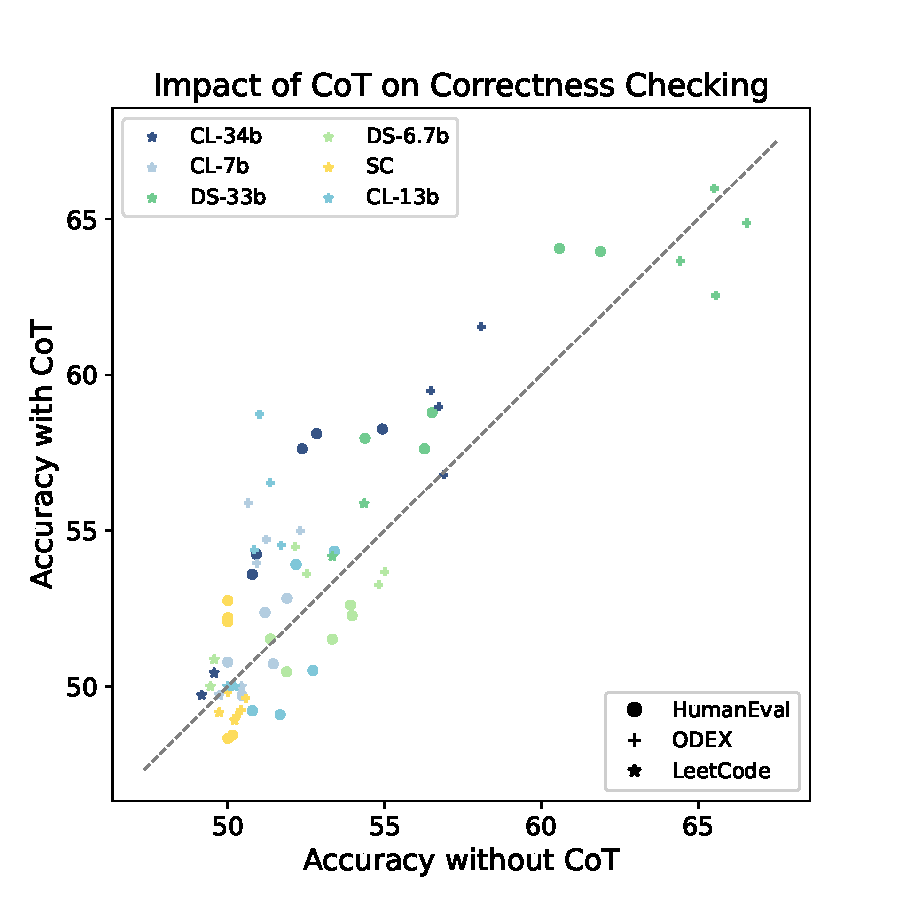
\includegraphics[width=0.5\textwidth]{figures_v2/appendix/misc/correctness_checking_nocot_cot.pdf}
    \caption{Models are slightly better when using CoT than without}
    \label{fig:correctness-checking-cot-impact}
\end{figure}

\textit{Execution Prediction}: For this task, we use the same prompt format as in \citep{gu2024cruxeval} with modified few-shot examples to better resemble our dataset format. We tested both CoT and non-CoT prompts, discovering that CoT did not help models other than GPT-3.5 and GPT-4. This is relatively consistent with the  results from \citet{gu2024cruxeval}\footnote{See their \href{https://crux-eval.github.io/leaderboard.html}{leaderboard}}, which only saw a 1.2\% improvement for Code Llama 34B and no improvement for Code Llama 13B. Therefore, we use CoT for GPT models, and non-CoT prompts for the others. The accuracy is calculated using pass@1 with $N=10, T=0.2$. 

\textit{Repair}: For this task, we base our prompt format on those employed in prior work by \citet{olausson2024repair}.
This prompt format is reminiscent of Chain-of-Thought in that it instructs the model to generate a textual explanation of what is wrong with the code, before generating the fixed version of the program.
Note that in our version of this prompt format, the model is not given any details as to what test test the program failed, and so has to relate the program to the natural language specification to debug it.
Unlike the other tasks, the prompt format we use for repair is zero-shot. 
Preliminary experiments indicated that this led to better results, particularly for smaller models which showed a tendency to debug the example program instead of the target. For the experiments with DeepSeek-based models, we replaced the HTML-style tags with Markdown-style tags (e.g., [PYTHON] $\to$ \`{}\`{}\`{}python).
Since repair requires generating a rather long answer, with both a textual explanation and a fixed version of the program, variance can be higher than in the other settings we consider.
To reduce this variance, we generate a large amount ($R=50$) of repair candidates for each counterfeit sample, using a temperature of $T=0.6$. We then average over all $5 \cdot 50 = 250$ samples to compute the mean success rate for each task, and also show a 95\% confidence interval on the mean.\footnote{Recall that our curated datasets contain 5 counterfeit samples per problem.}
Note that due to this increased computational burden, we do not carry out repair experiments for the full Cartesian product of models considered before, instead focusing on those open-source models that performed best on each dataset.

\subsection{Prompts}
\label{sec:prompts}
In this section, we list the HumanEval prompts. The prompts for other tasks can be found in our codebase \footnote{\url{https://github.com/update-after-deanonymization}}. Listings \ref{lst:correctness-checking-prompt-no-cot}, \ref{lst:correctness-checking-prompt-cot} show the correctness checking prompt without and with CoT, and Listings \ref{lst:execution-prompt-no-cot}, \ref{lst:execution-prompt-cot} show the execution prediction prompts. We give credit to \citet{gu2024cruxeval} and \citet{olausson2024repair} for their execution prediction and repair prompts.

\begin{lstlisting}[caption={Prompt for correctness checking (HumanEval)},label={lst:correctness-checking-prompt-no-cot}, style=boxed]
You will be given a Python coding problem with its specification and input/output examples in docstrings. 
Your goal is to determine whether the program exactly matches the specification. 
A correct program must be correct for all inputs, including hidden test cases not listed in the docstring.
In [ANSWER] and [/ANSWER] tags, write "Correct" if the program is correct, and "Incorrect" otherwise.

[PYTHON]
from typing import List


def is_at_least_zero(numbers: List[int]) -> bool:
    """ For a given list of numbers, checks if their sum is at least 0.
    >>> is_at_least_zero([1, -2, 3])
    True
    >>> is_at_least_zero([-1, -2, 2])
    False
    """
    return sum(numbers) >= 0
[/PYTHON]
[ANSWER]
Correct
[/ANSWER]

[PYTHON]
from typing import List


def identical_length(s: List[str]) -> bool:
    """ Check if in given list of strings, there exist two different
    strings with the same length.
    >>> identical_length(["abc", "def", "ghi"])
    True
    >>> identical_length(["abc", "gh"])
    False
    """
    for i in range(len(s)):
        for j in range(len(s)):
            if len(s[i]) == len(s[j]):
                return True
    return False
[/PYTHON]
[ANSWER]
Incorrect
[/ANSWER]
\end{lstlisting}

\begin{lstlisting}[caption={Prompt for correctness checking, CoT (HumanEval)},label={lst:correctness-checking-prompt-cot}, style=boxed]
You will be given a Python coding problem with its specification and input/output examples in docstrings. 
Your goal is to judge whether the program exactly matches the behavior specified in the docstring.
A correct program must be correct for all inputs, including hidden test cases not listed in the docstring.
First, think step by step about the program in [THOUGHT] and [/THOUGHT] tags.
In [ANSWER] and [/ANSWER] tags, write "Correct" if the program is correct, and "Incorrect" otherwise.

[PYTHON]
from typing import List


def is_at_least_zero(numbers: List[int]) -> bool:
    """ For a given list of numbers, checks if their sum is at least 0.
    >>> is_at_least_zero([1, -2, 3])
    True
    >>> is_at_least_zero([-1, -2, 2])
    False
    """
    return sum(numbers) >= 0
[/PYTHON]
[THOUGHT]
The function calculates the sum of a list of integers and checks if the sum is at least 0. The implementation uses Python's built-in sum function to calculate the total sum of the list and compares it with 0 using the >= operator. This approach should work correctly for any list of integers, including empty lists, where the sum would be 0, thus meeting the specification for all possible inputs.
[/THOUGHT]
[ANSWER]
Correct
[/ANSWER]

[PYTHON]
from typing import List


def identical_length(s: List[str]) -> bool:
    """ Check if in given list of strings, there exist two different
    strings with the same length.
    >>> identical_length(["abc", "def", "ghi"])
    True
    >>> identical_length(["abc", "gh"])
    False
    """
    for i in range(len(s)):
        for j in range(len(s)):
            if len(s[i]) == len(s[j]):
                return True
    return False
[/PYTHON]
[THOUGHT]
The program checks if any two strings in the list have the same length. However, it also compares each string with itself due to the loops' range, which means it will always find two strings (the same string compared with itself) with identical length, returning True incorrectly for any non-empty list. The correct approach should exclude the case where i equals j.
[/THOUGHT]
[ANSWER]
Incorrect
[/ANSWER]
\end{lstlisting}

\begin{lstlisting}[caption={Prompt for execution prediction (HumanEval)},label={lst:execution-prompt-no-cot}, style=boxed]
You are given a Python function and an assertion containing an input to the function.
Complete the assertion with a literal (no unsimplified expressions, no function calls) containing the output when executing the provided code on the given input.
Even if the function is incorrect or incomplete, give the output when executing the Python code as provided.
Assume all required imports have been included.
Do NOT output any extra information. Provide the full assertion with the correct output in [ANSWER] and [/ANSWER] tags, following the examples.

[PYTHON]
def add_one(number : int) -> int:
    return number + 2
assert add_one(17) == ??
[/PYTHON]
[ANSWER]
assert add_one(17) == 19
[/ANSWER]

[PYTHON]
def add_character_a(string : str) -> str:
    return string + "a"
assert add_character_a("x9j") == ??
[/PYTHON]
[ANSWER]
assert add_character_a("x9j") == "x9ja"
[/ANSWER]

[PYTHON]
{solution}
assert {input} == ??
[/PYTHON]
[ANSWER]
\end{lstlisting}

\begin{lstlisting}[caption={Prompt for execution prediction, CoT (HumanEval)},label={lst:execution-prompt-cot}, style=boxed]
You are given a Python function and an assertion containing an input to the function.
Complete the assertion with a literal (no unsimplified expressions, no function calls) containing the output when executing the provided code on the given input.
Even if the function is incorrect or incomplete, give the output when executing the Python code as provided.
Assume all required imports have been included. Think through the execution of the program in [THOUGHT] and [/THOUGHT] tags.
Provide the full assertion with the correct output in [ANSWER] and [/ANSWER] tags, following the examples.

[PYTHON]
def performOperation(s : str) -> str:
    s = s + s
    return "b" + s + "a"
assert performOperation("hi") == ??
[/PYTHON]
[THOUGHT]
Let's execute the code step by step:

1. The function performOperation is defined, which takes a single argument s.
2. The function is called with the argument "hi", so within the function, s is initially "hi".
3. Inside the function, s is concatenated with itself, so s becomes "hihi".
4. The function then returns a new string that starts with "b", followed by the value of s (which is now "hihi"), and ends with "a".
5. The return value of the function is therefore "bhihia".
[/THOUGHT]
[ANSWER]
assert performOperation("hi") == "bhihia"
[/ANSWER]

[PYTHON]
{solution}
assert {input} == ??
[/PYTHON]
[THOUGHT]
\end{lstlisting}

\begin{lstlisting}[caption={Prompt for (self-)repair (HumanEval)},label={lst:repair-prompt}, style=boxed]
=== system prompt ===
You are a helpful programming assistant and an expert Python programmer.
You are helping a user write a program.
The user has been given a function signature, along with a doc-string explaining its specification, and has then written an attempted implementation of the function.
Unfortunately, their code has some bugs and is not passing all of the hidden unit tests.

You will help the user by first giving a concise textual explanation of what is wrong with the code.
After you have pointed out what is wrong with the code, you will then generate a fixed version of the program.
Put your fixed program within code delimiters, for example:
[PYTHON]
# YOUR CODE HERE
[/PYTHON]
Do not change the function signature or doc-string in any way: they must be exactly as given by the user.

=== user prompt ===
### INCORRECT CODE
[PYTHON]
{code}
[/PYTHON]
The program does not pass all of the hidden test cases. Please fix it.
\end{lstlisting}
